\subsection{Evolutionäre Algorithmen}
"Unter evolutionären Algorithmen (EA) verstehen wir randomisierte Heuristiken, die Suchprobleme näherungsweise durch vereinfachende algorithmische Umsetzung von
Prinzipien der natürlichen Evolution zu lösen versuchen. Somit geben evolutionäre Algorithmen in der Regel weder eine Garantie bzgl. der benätigten Rechenzeit noch der Güte der ausgegebenen Lösung. Ein Suchproblem besteht darin, zu einer Zielfunktion ein Element aus deren Definitionsbereich zu finden, dessen Funktionswert möglichst gut ist. Darunter verstehen wir im Folgenden, wenn nicht ausdrücklich anders vermerkt, einen möglichst grossen Funktionswert, weshalb der Zielfunktions wert eines Elements auch als seine Fitness bezeichnet wird.\\

Der Aufbau eines evolutionären Algorithmus lässt sich dann grob wie folgt beschreiben: in jedem Schritt verwaltet er eine Menge fester Grösse von Suchpunkten, die so genannte Population, wobei jeder einzelne Suchpunkt auch als Individuum bezeichnet wird. Aus den Punkten der Population neue Punkte zu erzeugen, ist Aufgabe von Mutation und Rekombination. Dabei steht hinter der Mutation die Idee, jeweils nur ein einzelnes Individuum zufällig zu verändern, ohne dass andere Individuen dabei berücksichtigt werden. Durch Rekombination wird hingegen aus mehreren, meist zwei Individuen zufällig ein neues gebildet, das von diesen möglichst gute Eigenschaften übernehmen soll. Durch Mutation und Rekombination werden also neue Individuen (Kinder genannt) aus bestehenden Individuen (Eltern genannt) erzeugt. Beide Operatoren hängen oftmals stark von Zufallsentscheidungen ab. Jedoch fliesst in der Regel weder in Mutation noch Rekombination der Zielfunktionswert der Individuen ein.\\

Die Zielfunktion beeinflusst nur die Selektion. Dieser Operator wählt Individuen der Population aus, sei es zur Auswahl der Eltern für eine Rekombination oder Mutation oder, um aus der Menge von Eltern und Kindern die nächste Population zu wählen, was den Übergang zur nächsten Generation darstellt. Dadurch, dass die Selektion Punkte mit höherem Zielfunktionswert mit grösserer Wahrscheinlichkeit auswählt, soll erreicht werden, dass nach und nach immer bessere Punkte gefunden werden." \cite{droste}

\begin{figure}[h]
  \centering
  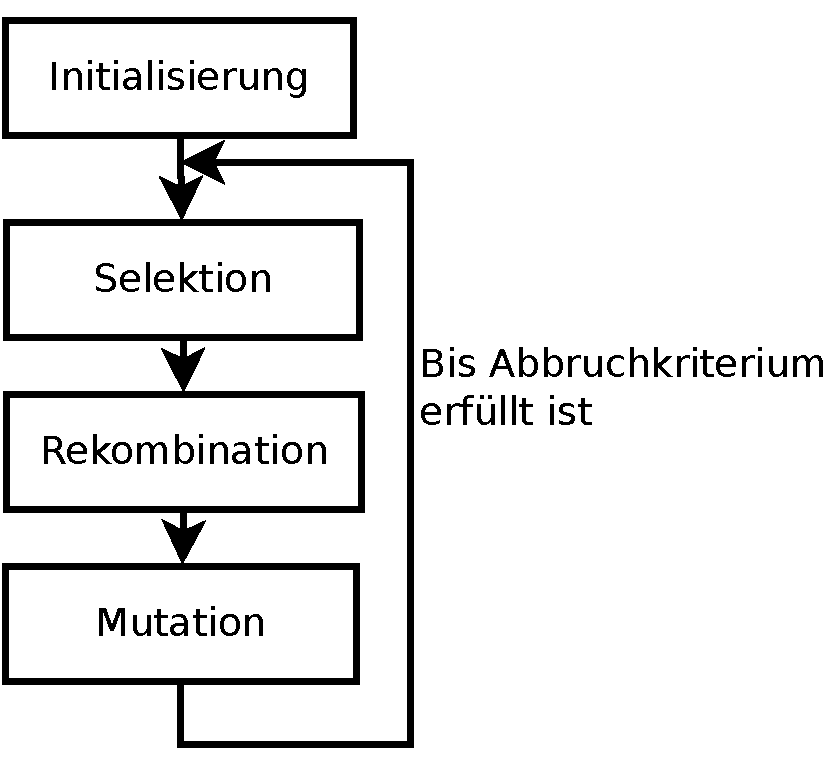
\includegraphics{images/evolutionaerer_algorithmus.pdf}
  \caption[Evolutionärer Algorithmus]{Evolutionärer Algorithmus}
  \label{fig:endlicher_automat}
\end{figure}

\subsubsection{Anwendung auf unser Problem}
Unser Problem der Findung von regulären Automaten welche die selbe Sprache akzeptieren wie ein gegebener regulärer Ausdruck läst sich wie mit einigen Anpassungen in diesem Standartmodell eines evolutionären Algorithmus abbilden.

\paragraph{Initialisierung}
In der Initialisierungsphase werden wir eine Population von Automaten zufällig erzeugen. Das heisst wir erzeugen eine Zufällige Anzahl von Zuständen, verbinden diese Zufällig und setzen einen zufälligen Start und zufällige Akzeptierende Zustände.\\

\selektion{Selektion}
Es werden jeweils diejenigen Automaten selektiert welche eine höhere Fitness aufweisen. Es werden verschiedene Ansätze zur Selektion implementiert und es wird deren Konvergenzverhalten analysiert.\\ 

\paragraph{Fitness}
Die Fitness von Automaten bestimmen wir in dem wir ihn mit Wörtern füttern und die Ausgabe mit der soll Ausgabe vergleichen. Die Soll Ausgabe können wir anhand des gegebenen regulären Ausdrucks einfach bestimmen. Der Wert der Fitnessfunktion entspricht dann der Summe der richtig akzeptierten und richtig nicht akzeptierten Wörtern aus unserer \textit{Problemmenge}.\\

\paragraph{Problemmenge}
Die Problemmenge ist eine Menge von Tupeln ($Wort$, $Soll Ausgabe$) welche verwendet wird um die Fitness von Automaten zu bestimmen. Im Rahmen dieser Arbeit werden unter anderem Verschiedene Ansätze zur Erzeugung und zum Verhalten solcher Problemmengen ausprobiert. Dabei wird das Konvergenzverhalten des evolutionären Algorithmus untersucht.\\

\paragraph{Rekombination}
Wenn man zwei endliche Automaten graphisch zusammenfügt, wird der resultierende Automat ein komplett anderes Verhalten aufweisen als die beiden Eltern. Deshalb verzichten wir auf die rekombination im herkömmlichen Sinne. Wir klonen jeweils die selektierten Automaten und \textit{mutieren} die so entstandenen Kinder.\\

\paragraph{Mutation}
Bei der Mutation soll jeweils eine zufällige Veränderung an einem Automaten durchgeführt werden. Wir haben uns auf folgende Mutationen festgelegt:\\
\begin{enumerate}
	\item einen Zustand hinzufügen
	\item einen Zustand entfernen
	\item eine Verbindung zwischen zwei Zuständen ändern
	\item einen nicht akzeptierenden Zustand zu einem akzeptierenden Zustand umwandeln
	\item einen akzeptierenden Zustand zu einem nicht akzeptierenden Zustand umwandeln
\end{enumerate}